\documentclass[11pt]{article}
\usepackage[a4paper,margin=1in]{geometry}
\usepackage{amsmath,amssymb,amsthm}
\usepackage{tikz}
\usetikzlibrary{decorations.pathreplacing}
\usepackage{xcolor}
\usepackage[hidelinks]{hyperref}
\hypersetup{pdftitle={The easiest dice to tell apart},pdfauthor={Vamshi Jandhyala}}
\setlength{\parskip}{0.4em}
\setlength{\parindent}{0pt}

\newtheorem{theorem}{Theorem}
\newtheorem{proposition}{Proposition}
\newtheorem{lemma}{Lemma}
\newtheorem{corollary}{Corollary}
\theoremstyle{remark}
\newtheorem*{remark}{Remark}

\definecolor{inkblue}{RGB}{40,76,105}
\definecolor{softblue}{RGB}{226,235,243}
\definecolor{rust}{RGB}{153,70,45}

\newcommand{\ov}{\operatorname{ov}}

\title{The easiest dice to tell apart}
\author{Vamshi Jandhyala}
\date{}

\begin{document}
\maketitle
\vspace{-2em}

\begin{abstract}
Two loaded dice have $k$ faces, and no face of either die comes up with probability more than $r$. Both
are rolled $n$ times, and we must guess which die produced the sequence. We find the pair that is easiest to
tell apart, for every $k$, $r$ and $n$: a staircase $(r,\dots,r,1-mr,0,\dots,0)$, $m=\lfloor 1/r\rfloor$,
against its own reversal. This answers a question on Mathematics Stack Exchange, which asked for $k=4$ and
$1/3<r<1/2$. For that case we also find every pair that does as well, except when $n=2$, where we exhibit a
one-parameter family. The proof compares the dice face set by face set at every exchange rate, which
takes three lines for one roll; a standard argument then handles $n$ rolls. Every step is checked in the Lean
proof assistant.
\end{abstract}

\section{The question}

Let $p=(p_1,\dots,p_k)$ and $q=(q_1,\dots,q_k)$ be the face probabilities of two dice. Roll one of them $n$
times. A sequence of faces $w=(i_1,\dots,i_n)$ has probability $P(w)=p_{i_1}\cdots p_{i_n}$ under the first
die and $Q(w)=q_{i_1}\cdots q_{i_n}$ under the second. The \emph{overlap}
\[
\ov_n(p,q)=\sum_{w}\min\bigl(P(w),Q(w)\bigr)
\]
measures how hard the dice are to tell apart. If each die is chosen with probability $\frac12$, the best
possible guess is wrong with probability exactly $\frac12\ov_n(p,q)$: for each $w$, guess the die that makes
$w$ more likely, and you are wrong with probability $\frac12\min(P(w),Q(w))$.

Identical dice have overlap $1$, and dice with no face in common have overlap $0$. The question~\cite{MSE}
puts a cap on how loaded the dice may be: every $p_i$ and every $q_i$ is at most $r$. For $k=4$ and
$\frac13<r<\frac12$, how small can the overlap be? The asker proved $\ov_n\ge(2-4r)^n$, and computed the overlap of the pair
\[
p=(r,\;s,\;r,\;0),\qquad q=(0,\;r,\;s,\;r),\qquad s=1-2r,
\]
which bounds the least overlap from above. At $n=2$ and $r=\frac25$ the two bounds are $\frac4{25}$ and $\frac6{25}$. Stop and
try to decide which is the truth before reading on.

The pair is the answer, and it is a case of a pattern that holds for every number of faces and every cap.
Write $m=\lfloor1/r\rfloor$ and define the \emph{staircase} and its reversal
\[
p^*=(\underbrace{r,\dots,r}_{m},\;1-mr,\;0,\dots,0),\qquad q^*_i=p^*_{k+1-i}.
\]
(When $1/r$ is an integer, $1-mr=0$.) For $k=4$ and $\frac13<r<\frac12$ this is $p^*=(r,r,s,0)$ and
$q^*=(0,s,r,r)$, the asker's pair with two faces renamed (Figure~\ref{fig:stair}).

\begin{theorem}\label{thm:main}
Let $kr\ge1$, so that capped dice exist. For every $n\ge1$ and every choice of capped dice, which may even
differ from roll to roll, the overlap of the $n$ rolls is at least $\ov_n(p^*,q^*)$.
\end{theorem}

\begin{corollary}\label{cor:asker}
For $k=4$ and $\frac13<r<\frac12$ the least overlap is the asker's bound,
\[
C_n(r)=2\sum_{j>n/2}\binom nj s^jr^{n-j}\;+\;[n\text{ even}]\binom n{n/2}(rs)^{n/2}.
\]
In particular $C_2(\frac25)=\frac6{25}$.
\end{corollary}

The formula is the asker's evaluation of their pair~\cite{MSE}, which we have checked for $n\le6$; it comes from
sorting the words of the staircase pair: a word containing face
$(r,0)$ or face $(0,r)$ contributes nothing, and a word made of $j$ faces $(s,r)$ and $n-j$ faces $(r,s)$
contributes $\min(s^jr^{n-j},r^js^{n-j})$.

\begin{figure}[ht]
\centering
% Staircase pair for k = 4, r = 2/5: p* above the axis, q* below; the first a = 2 faces bracketed.
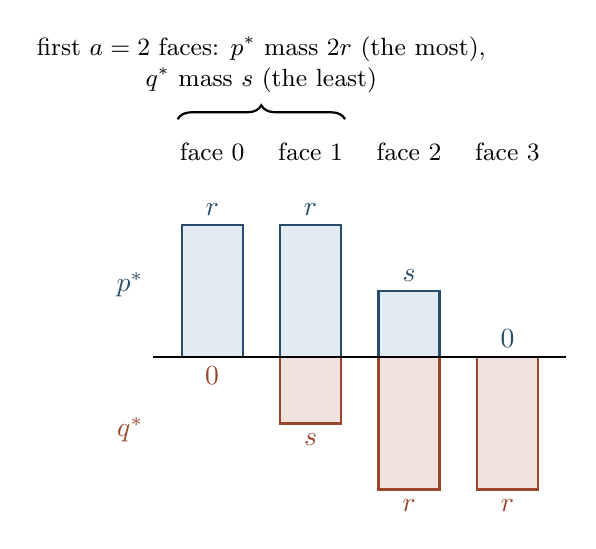
\begin{tikzpicture}[x=1.25cm,y=4.2cm]
  \def\w{0.62}
  % p* bars (up)
  \foreach \i/\h/\lab in {0/0.4/{$r$},1/0.4/{$r$},2/0.2/{$s$}} {
    \fill[softblue,draw=inkblue,thick] (\i-\w/2,0) rectangle (\i+\w/2,\h);
    \node[above,inkblue] at (\i,\h) {\lab};
  }
  \node[above,inkblue] at (3,0) {$0$};
  % q* bars (down)
  \foreach \i/\h/\lab in {1/0.2/{$s$},2/0.4/{$r$},3/0.4/{$r$}} {
    \fill[rust!15,draw=rust,thick] (\i-\w/2,0) rectangle (\i+\w/2,-\h);
    \node[below,rust] at (\i,-\h) {\lab};
  }
  \node[below,rust] at (0,0) {$0$};
  \draw[thick] (-0.6,0) -- (3.6,0);
  \node[left,inkblue] at (-0.6,0.22) {$p^*$};
  \node[left,rust] at (-0.6,-0.22) {$q^*$};
  \foreach \i in {0,1,2,3} \node[font=\small] at (\i,0.62) {face \i};
  % bracket over the first two faces
  \draw[decorate,decoration={brace,amplitude=5pt},thick] (-0.35,0.72) -- (1.35,0.72)
    node[midway,above=6pt,font=\small,align=center] {first $a=2$ faces: $p^*$ mass $2r$ (the most),\\ $q^*$ mass $s$ (the least)};
\end{tikzpicture}

\caption{The staircase pair for $k=4$, $r=\frac25$, $s=\frac15$: $p^*$ above the line, $q^*$ below. Any two
faces carry at most $2r$ of a capped die. Any two faces carry at least $1-2r=s$ of a capped die, because the
other two carry at most $2r$. The first two faces of the staircase pair meet both limits at once. The same
holds for the first $a$ faces, for every $a$.}
\label{fig:stair}
\end{figure}

\section{Overlap as an excess}

For $a,b\ge0$, $\min(a,b)=a-(a-b)^+$, where $x^+=\max(x,0)$. Since the $P(w)$ add up to $1$,
\[
\ov_n=1-\sum_w\bigl(P(w)-Q(w)\bigr)^+ .
\]
So a small overlap means a large \emph{excess} of $P$ over $Q$. The proof needs the excess at every
exchange rate, so for $u,v\ge0$ set
\[
g_{p,q}(u,v)=\sum_{i=1}^k\bigl(u\,p_i-v\,q_i\bigr)^+ .
\]
Read it as a bet on faces. Choose a set $A$ of faces; gain $u$ for each unit of $p$ on $A$ and lose $v$ for each
unit of $q$ on $A$. The best set is $A=\{i:u\,p_i>v\,q_i\}$, so
\begin{equation}\label{eq:bet}
g_{p,q}(u,v)=\max_{A}\bigl(u\,p(A)-v\,q(A)\bigr),\qquad p(A)=\sum_{i\in A}p_i .
\end{equation}
For $n$ rolls, with die $(p^{(j)},q^{(j)})$ at roll $j$, define $G(u,v)=\sum_w\bigl(u\,P(w)-v\,Q(w)\bigr)^+$ in
the same way. The overlap is $1-G(1,1)$.

\section{One roll}

\begin{lemma}\label{lem:sets}
Let $p$ and $q$ be capped dice and let $A$ be a set of $a$ faces. Then
\[
p(A)\le\min(1,\,ar),\qquad q(A)\ge\max\bigl(0,\,1-(k-a)r\bigr).
\]
The first $a$ faces of the staircase pair meet both bounds: $p^*(\{1,\dots,a\})=\min(1,ar)$ and
$q^*(\{1,\dots,a\})=\max(0,1-(k-a)r)$.
\end{lemma}

\begin{proof}
Each face carries at most $r$, and the whole die carries $1$; this gives the bound on $p(A)$. The other
$k-a$ faces carry at most $(k-a)r$ of $q$, which gives the bound on $q(A)$. For the staircase, the partial sums
of $p^*$ are $r,2r,\dots,mr$, then $1$ for ever, which is $\min(1,ar)$. The first $a$ faces of $q^*$ are the
last $a$ faces of $p^*$, which carry $1-\min(1,(k-a)r)=\max(0,1-(k-a)r)$.
\end{proof}

\begin{proposition}\label{prop:one}
For capped dice $p,q$ and all $u,v\ge0$, $g_{p,q}(u,v)\le g_{p^*,q^*}(u,v)$.
\end{proposition}

\begin{proof}
Take the best set $A$ in~\eqref{eq:bet} and let $a=|A|$. By Lemma~\ref{lem:sets}, the bet on $A$ gains at most
$u\min(1,ar)-v\max(0,1-(k-a)r)$. The staircase pair gains exactly that by betting on its first $a$ faces, and
its best bet gains at least as much.
\end{proof}

The staircase pair wins at every exchange rate at once, and that is what the next step needs: when we go from
one roll to many, each roll is judged at a rate that the other rolls set.

\section{Many rolls}

Split a word into its first face $i$ and the rest $x$. Then $P(w)=p_i P'(x)$ and $Q(w)=q_i Q'(x)$, where
$P',Q'$ belong to the last $n-1$ rolls, and the excess can be summed in either order:
\begin{equation}\label{eq:split}
G(u,v)=\sum_i G'\bigl(u\,p_i,\;v\,q_i\bigr)=\sum_x g_{p,q}\bigl(u\,P'(x),\;v\,Q'(x)\bigr).
\end{equation}
The first form says the last $n-1$ rolls are judged at the rate $(u\,p_i,v\,q_i)$ that the first roll
sets; the second says the first roll is judged at the rate $(u\,P'(x),v\,Q'(x))$ that the others set.

\begin{proof}[Proof of Theorem~\ref{thm:main}]
We show $G(u,v)\le G^*(u,v)$ for all $u,v\ge0$, where $G^*$ belongs to $n$ rolls of the staircase pair, by
induction on $n$. For $n=0$ both sides are $(u-v)^+$. For the step, use the first form of~\eqref{eq:split}
and the induction hypothesis to replace the last $n-1$ rolls by staircase rolls; then use the second form and
Proposition~\ref{prop:one}, at each rate $(u\,P'(x),v\,Q'(x))$, to replace the first roll
(Figure~\ref{fig:rolls}). Neither step decreases the excess. At $u=v=1$ this is the theorem.
\end{proof}

\begin{figure}[ht]
\centering
% Replacing the rolls one at a time: each row's excess is at most the next row's.
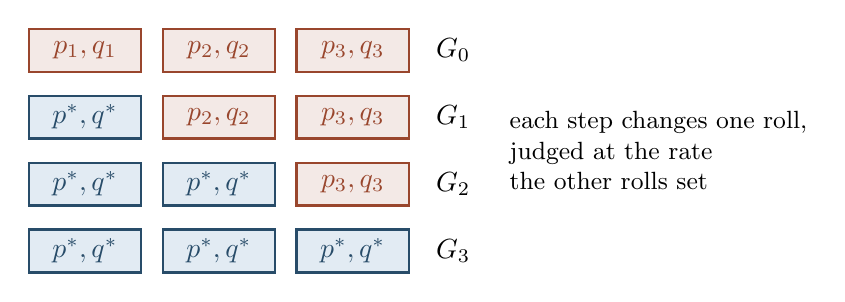
\begin{tikzpicture}[x=1.7cm,y=0.85cm]
  \foreach \row in {0,1,2,3} {
    \foreach \j in {1,2,3} {
      \ifnum\j>\row
        \fill[rust!12,draw=rust,thick] (\j-0.42,-\row-0.32) rectangle (\j+0.42,-\row+0.32);
        \node[rust] at (\j,-\row) {$p_\j,q_\j$};
      \else
        \fill[softblue,draw=inkblue,thick] (\j-0.42,-\row-0.32) rectangle (\j+0.42,-\row+0.32);
        \node[inkblue] at (\j,-\row) {$p^*,q^*$};
      \fi
    }
    \node[anchor=west] at (3.55,-\row) {$G_{\row}$};
  }
  \node[anchor=west,font=\small,align=left] at (4.1,-1.5) {each step changes one roll,\\ judged at the rate\\ the other rolls set};
\end{tikzpicture}

\caption{Three rolls, with excesses $G_0\le G_1\le G_2\le G_3$. Replacing one roll by the staircase pair cannot
decrease the excess, because the staircase pair wins at every rate (Proposition~\ref{prop:one}).}
\label{fig:rolls}
\end{figure}

\begin{remark}
This second step is standard. Proposition~\ref{prop:one} says that $(p^*,q^*)$ is more informative than
every capped pair in Blackwell's sense: domination at every rate is equivalent to one experiment being a
garbling of the other (Blackwell~\cite[Theorem~10]{Bla53}, in the form of~\cite[Theorem~2.5]{KOV15}), and the
induction above is the familiar fact that products keep that order. The same
pattern of one dominant experiment, then its $k$-fold product, is how Kairouz, Oh and Viswanath prove their
optimal composition theorem for differential privacy~\cite[Section~3.1]{KOV15}. What is particular here is
that the capped dice have a dominant pair at all, and Lemma~\ref{lem:sets} shows why: one chain of nested
sets is extreme for both dice at once.
\end{remark}

\section{Who else does as well, for four faces}

From here on $k=4$, $\frac13<r<\frac12$ and $s=1-2r$, so $0<s<r$. Relabelling faces does not change the
overlap, so every pair with one face of each kind $(r,0)$, $(r,s)$, $(s,r)$, $(0,r)$ reaches $C_n(r)$.

\begin{theorem}\label{thm:eq}
Let $p,q$ be capped dice with four faces and $\ov_n(p,q)=C_n(r)$.
\begin{enumerate}
\item[(a)] For $n=1$ this happens exactly when $\max(p_i,q_i)=r$ for every face.
\item[(b)] For $n\ge3$ it happens only for the four kinds of face above, one of each.
\end{enumerate}
For $n=2$ it also happens for $p=(r,\,r,\,x,\,s-x)$, $q=(0,\,s,\,r,\,r)$ with $0\le x\le s$.
\end{theorem}

Part (a) is a line of algebra: $\ov_1=\sum_i\min(p_i,q_i)=2-\sum_i\max(p_i,q_i)\ge 2-4r$. The family for
$n=2$ is a direct computation of $G(1,1)$ through~\eqref{eq:split}; it equals
$r+2r^2-s^2+rs$ for every $x$. We have not proved that this family, with its relabellings and with $p$ and $q$
swapped, is the whole answer for $n=2$.

For (b), equality forces equality all the way along the chain in the proof of Theorem~\ref{thm:main}. Since
each step there compares sums term by term, every term must agree.

\begin{lemma}\label{lem:rates}
If $\ov_n(p,q)=C_n(r)$, then $g_{p,q}=g_{p^*,q^*}$ at the rate $(P^*(x),Q^*(x))$ for every word $x$ of
$n-1$ staircase rolls, and at $(p_i P^*(x),q_i Q^*(x))$ for every face $i$ and every word $x$ of $n-2$
staircase rolls.
\end{lemma}

The next lemma says what equality at one rate means. Write $B(a)=u\min(1,ar)-v\max(0,1-(4-a)r)$ for the bound
on a bet over $a$ faces from Lemma~\ref{lem:sets}. With four faces the five values are
\[
B(0)=0,\quad B(1)=ur,\quad B(2)=2ur-vs,\quad B(3)=u-v(1-r),\quad B(4)=u-v .
\]

\begin{lemma}\label{lem:tight}
If $u,v>0$ and $g_{p,q}(u,v)=g_{p^*,q^*}(u,v)$, let $A=\{i:u\,p_i>v\,q_i\}$ and $a=|A|$. Then $B(a)$ is the
largest of the five values, $p(A)=\min(1,ar)$ and $q(A)=\max(0,1-(4-a)r)$.
\end{lemma}

\begin{proof}
In the proof of Proposition~\ref{prop:one} every inequality must be an equality, and the two inequalities of
Lemma~\ref{lem:sets} are each multiplied by a positive number.
\end{proof}

\begin{proof}[Proof of Theorem~\ref{thm:eq}(b)]
Write $t=v/u$. Three rates pin the pair down.

\emph{A high rate.} The word of $n-1$ faces $(s,r)$ gives $t=(r/s)^{n-1}>r/s$. Then $B(1)$ is the unique
largest value, so $|A|=1$, $p(A)=r$ and $q(A)=0$: some face is $(r,0)$.

\emph{A low rate.} The word of $n-1$ faces $(r,s)$ gives $t=(s/r)^{n-1}<s/r$. Now $B(3)$ is the unique largest,
so $p(A)=1$ and $q(A)=1-r$. The face outside $A$ is $(0,r)$.

\emph{A middle rate.} The other two faces carry $1-r$ of each die, so each of their $p$ and $q$ values lies
between $s$ and $r$, and one of them, say $(p_i,q_i)$, has $p_i\ge q_i$.

If $n$ is odd, the word with $\frac{n-1}2$ faces of each kind $(r,s)$, $(s,r)$ gives $t=1$. Then $B(2)$ is the
unique largest, so $A$ is two faces with $p=r$ on both and $q(A)=s$. Face $(r,0)$ is one of them, so the
other is $(r,s)$, and the remaining face is $(s,r)$.

If $n$ is even, use the face $i$ with $p_i\ge q_i$ and the balanced word of $n-2$ rolls: this gives
$t=q_i/p_i$, which lies between $s/r$ and $1$. There $B(2)$ is largest, tied with $B(3)$ only when
$t=s/r$. If $|A|=3$, then $q_i/p_i=s/r$ with $p_i\le r$ and $q_i\ge s$, so $(p_i,q_i)=(r,s)$. If $|A|=2$, then
$A$ has $p=r$ on both faces and $q=r$ on both faces outside $A$; it contains the face $(r,0)$ and not the face
$(0,r)$. Suppose face $i$ were outside $A$. Then $q_i=r$, hence $p_i=r$, and the fourth face would be the
second face of $A$, with $p=r$; but the four values of $p$ would then add up to $3r>1$. So
$A=\{(r,0),i\}$ and $q_i=s-0=s$. Either way face $i$ is $(r,s)$, and the fourth face is $(1-2r,1-r-s)=(s,r)$.
\end{proof}

\paragraph{Verification.} Every theorem and lemma is proved in Lean~4 with Mathlib~\cite{mathlib}, using only
the standard axioms: Lemma~\ref{lem:sets} and Proposition~\ref{prop:one} for every $k$ and $r$, the product step
for dice that change from roll to roll, Corollary~\ref{cor:asker} as the statement that the asker's pair has the
least overlap, Lemmas~\ref{lem:rates} and~\ref{lem:tight}, and Theorem~\ref{thm:eq} with its $n=2$ family. The
closed form in Corollary~\ref{cor:asker} is checked by program, not in Lean. Python programs check, in exact rational arithmetic, the
one-roll domination for $k\le7$ at every breakpoint, the many-roll inequality for random mixed dice, the
closed form in Corollary~\ref{cor:asker} for $n\le6$, and the equality cases for $n\le4$; deliberately wrong
variants fail each check. An independent program, sharing no code with the others, searches numerically for
pairs with a smaller overlap and finds none. Everything is at
\url{https://github.com/jvvk/mathematics/tree/main/easiest-dice}.

\paragraph{Acknowledgements.} Dang Dang asked the question on Mathematics Stack Exchange~\cite{MSE} and found
the extremal pair. Anthropic's Claude (Opus~5.5) was used to find the argument, write the Lean formalisation
and the programs, and draft this text. The author takes responsibility for the content.

\begin{thebibliography}{9}
\bibitem{MSE} Dang Dang, Prove or disprove $\sum\min\{x_{i_1}\cdots x_{i_n},y_{i_1}\cdots y_{i_n}\}\ge(2+z)^{-n}$,
Mathematics Stack Exchange question 5149864 (20 September 2026),
\url{https://math.stackexchange.com/q/5149864}, accessed 10 October 2026.
\bibitem{Bla53} D.~Blackwell, Equivalent comparisons of experiments, \emph{Ann. Math. Statist.} \textbf{24}
(1953) 265--272, \href{https://doi.org/10.1214/aoms/1177729032}{doi:10.1214/aoms/1177729032}.
\bibitem{KOV15} P.~Kairouz, S.~Oh and P.~Viswanath, The composition theorem for differential privacy, in
\emph{Proceedings of the 32nd International Conference on Machine Learning}, PMLR \textbf{37} (2015) 1376--1385.
\bibitem{mathlib} The mathlib Community, The Lean mathematical library, in \emph{Proceedings of the 9th ACM
SIGPLAN International Conference on Certified Programs and Proofs (CPP 2020)}, 367--381,
\href{https://doi.org/10.1145/3372885.3373824}{doi:10.1145/3372885.3373824}.
\end{thebibliography}

\bigskip
\noindent Vamshi Jandhyala, London, UK.

\end{document}
